\section{Data and assumptions for scenarios} \label{Appendix}
\begin{table}[!ht]
	\caption{Data for initial condition.}
	\vspace{0.1in}
	\begin{tabularx}{1.2\textwidth}{p{0.35\textwidth} p{0.25\textwidth} p{0.2\textwidth} p{0.25\textwidth}}
		\hline
\textbf{Technology} & \textbf{\gls{lcoe}} & \textbf{Emission} & \textbf{Year of total}\\
  & (USD/kWh) & \textbf{Coefficients} (gCO$_2$-eq. /kWh) & \textbf{retirement} \\
\hline
Coal & 0.06 & 943 & 2030 \\
\gls{lng} & 0.08 & 599 & 2030 \\
Oil & 0.39 & 738 & 2030 \\
Nuclear & 0.11 & 21 & 2069 \\
Hydro & 0.05 & 11 & N.A. \\
Geothermal & 0.12 & 13 & N.A. \\
Wind & 0.11 & 25 & 2040 \\
Solar & 0.15 & 37 & 2040 \\
\hline 
\end{tabularx}
\label{init-eco}
\end{table}

\begin{figure}[h] 
\centering
\label{ic-elc}
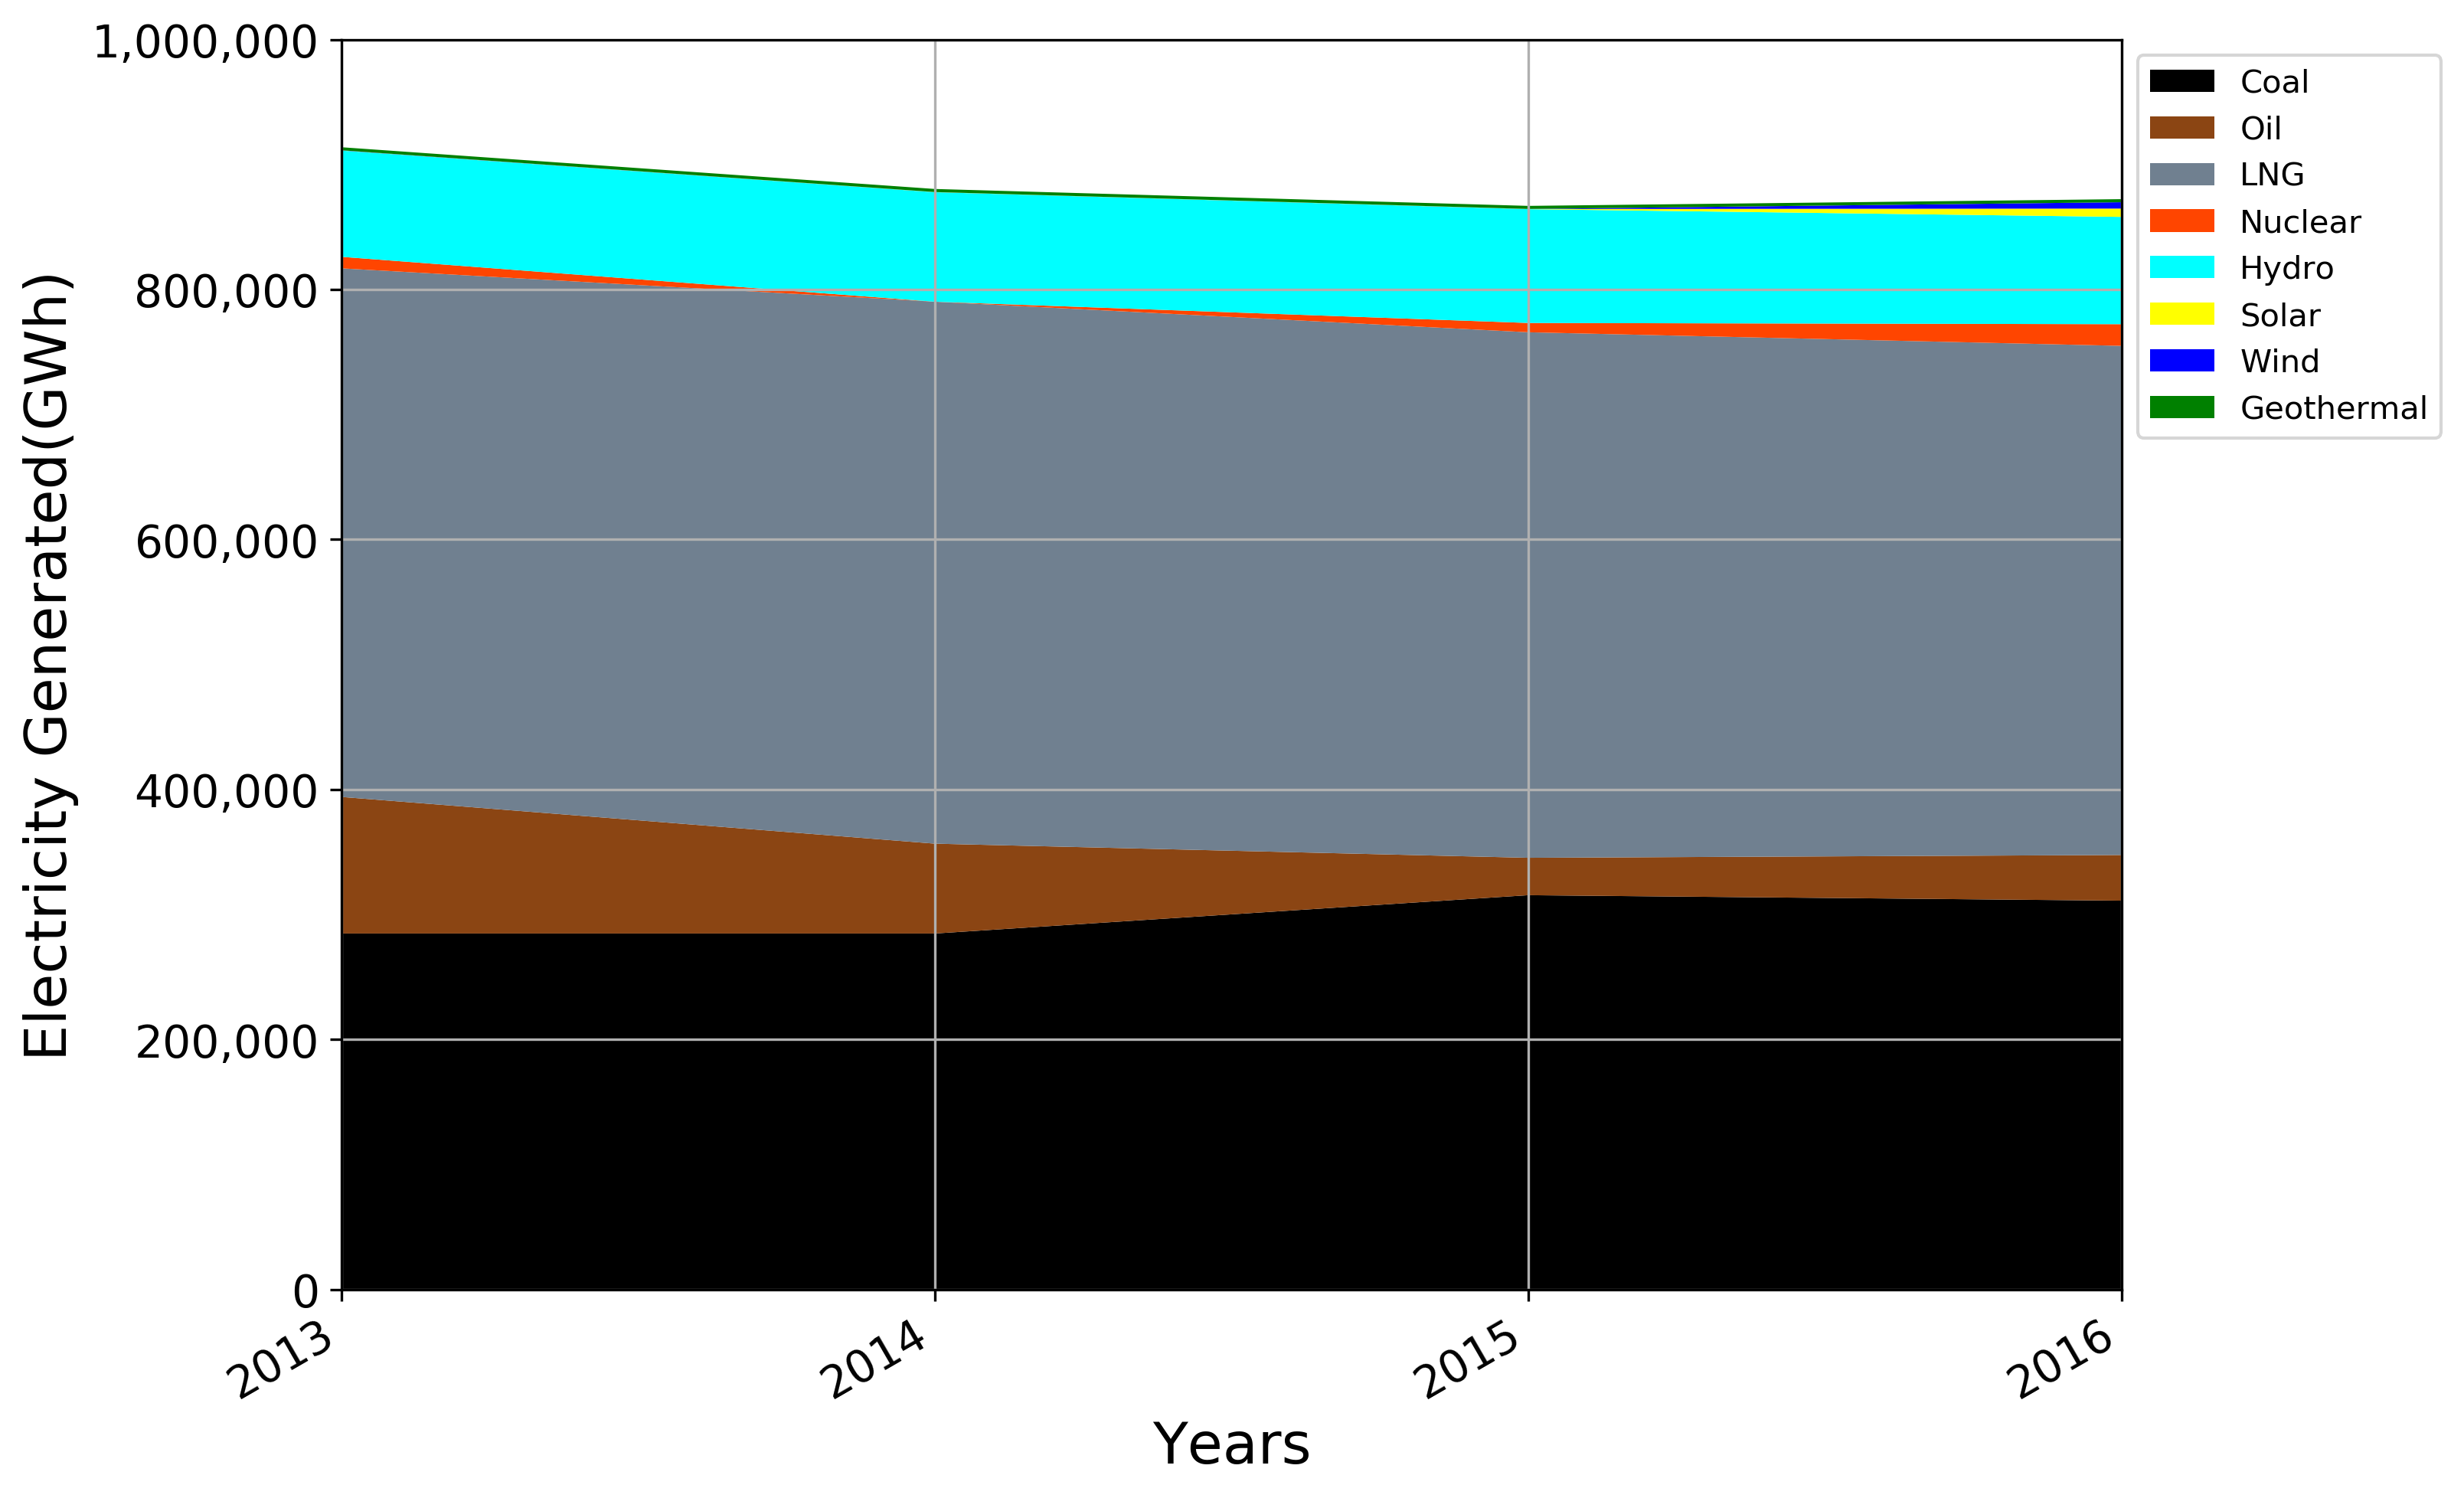
\includegraphics[scale=0.5]{figures/IC}
\caption{Electricity generation that defines the initial condition of the model.}
\end{figure}

\begin{table}[!ht]
	\caption{Initial condition CO$_2$ emissions compared to the model and data from the Carbon Trust.}
	\vspace{0.1in}
	\begin{tabularx}{\textwidth}{p{0.08\textwidth} p{0.35\textwidth} p{0.35\textwidth} p{0.15\textwidth}}
		\hline
\textbf{Year} & \textbf{Model Emissions} & \textbf{Actual Emissions} & \textbf{Error} \\
  & Mt CO$_2$-eq. & Mt CO$_2$-eq. &  \\
\hline
2013 & 603.62 & 592.4 & 1.89 \% \\
2014 & 582.27 & 572.6 & 1.69 \% \\
2015 & 572.53 & 560.3 & 2.18 \% \\
2016 & 565.94 & 552.8 & 2.38 \% \\
\hline 
	\end{tabularx}
\label{ic-co2}
\end{table}

\begin{landscape}
\begin{longtable}{ |*{8}{c|} }
\caption{Economic data for modelled technologies.}\\
\hline
\textbf{Technology} & \textbf{Capital} & \textbf{Fixed} & \textbf{Variable} & \textbf{Lifespan} & \textbf{Capacity Factor/} & \textbf{Emission} & \textbf{Year} \\
\textbf{name} & \textbf{Cost} & \textbf{\gls{OM}} & \textbf{\gls{OM}} &  & \textbf{Efficiency} & \textbf{Coefficient} & \textbf{available} \\
 & MUSD/GW & MUSD/GW & MUSD/GWh & Years  &  & gCO$_2$/kWh  &  \\
\hline
\endhead  % header material
\hline
\endfoot  % footer material
\hline
\endlastfoot
\gls{USC} & 3661 & 40.41 & 0.045 & 40 & CF=0.55 & 820 & 2017 \\
\gls{lng} & 1079 & 14 & 0.0025 & 30 & CF=0.55 & 490 & 2017 \\
Nuclear & 6317 & 121.13 & 2.36 & 60 & CF=0.6-0.95 & 12 & 2017 \\
Li-ion Storage & 1876 (2017) & 10 & 0.3 & 10 & Eff=0.86 & 151(2017) & 2017 \\
 & 1446 (2025) &  &  &  &  & 87(2050) &  \\
Solar & 1307(2017) & 15.19 & 0  & 25 & CF=0.14 & 37 & 2017 \\
 & 615(2050) & & & & & &  \\
Onshore Wind & 3454(2017) & 136.37 & 0 & 25 & CF=0.25(2017) & 20(2017) & 2017 \\
 & 2406(2050) &  &  &  & CF=0.35(2050) & 7 (2040) &  \\
Offshore Wind(Fixed) & 7772(2017) & 341 & 0 & 25 & CF=0.3(2017) & 25(2017) & 2017 \\
 & 3381(2050) &  &  & & CF=0.40(2050) & 11(2050) &  \\
Offshore Wind(Floating) & 12897(2017) & 423 & 0 & 25 & CF=0.35(2017) & 25(2017) & 2017 \\
 & 5610(2050) &  &  &  & CF=0.45(2050) & 11(2050) &  \\
LNG-CCS(90\%) & 2626(2022) & 27.484 & 0.0494 & 30 & CF=0.12-0.4(2017) & 94 & 2022 \\
 & 1422(2050) &  & &  &  &  & \\
USC-CCS(90\%) & 5252(2023) & 59 & 0.078 & 40 & CF=0.27-0.32(2017) & 236.5 & 2023 \\
 & 4091(2050) &  &  &  &  &  & \\
Emerging Solar & 4600(2017) & 15.19 & 0 & 25 & Eff=0.22(2017) & 22(2017) & 2017 \\
  & 600(2050) &  &  &  &Eff=0.3(2030)  & 13(2040) &  \\
\gls{AEC} & 1500(2022) & 8 & 0.0004 & 11(CF=0.9) & Eff=0.7 & 1.29 & 2022\\
 & 850(2030) &  &  &  &  & &  \\
\gls{PEMEC} & 3500(2022) & 8 & 0.0004 & 7 (2022)(CF=0.9) & Eff=0.75(2022) & 8.7(2022) & 2022\\
 & 1500(2030) &  & 11(2050)  &  & Eff=0.82(2030) & 0.456(2050)  &  \\
 & 400(2050) &  &  &  & &  &  \\
\gls{SOEC} & 6000(2030) & 8 & 0.0004 & 2 (2030)(CF=0.9) & Eff=0.9 & 5.4(2030) & 2030\\
 & 1000(2050) &  &  & 7 (2050) &  & 1.08(2050) & \\
 & 400(2070) &  &  & 11 (2070) &  & 0.72(2070) & \\
Gas Reforming & 763 & 6.21 & 0.04 & 30  & Eff=0.7 & 356.6 & 2022\\
Gas Reforming-CCS(70\%) & 1200 & 8 & 0.065 & 30 & Eff=0.56 & 179 & 2022\\
\gls{PEMFC} & 7399(2022) & 30.65 & 0.59 & 7 (CF=0.9) & Eff=0.49 & 1.087(2022) & 2022\\
 & 4000(2030) &  &  &  &  & 0.65(2030) &  \\
 & 3000(2035) &  &  &  &  &  &  \\
\gls{SOFC} & 7399(2030) & 30.65 & 0.59 & 10 (CF=0.9) & Eff=0.7 & 2.11(2030) & 2030\\
 & 4000(2035) &  &  &  &  & 1.27(2040) &  \\
 & 3000(2040) &  &  &  &  & &  \\
\gls{PWS} & 14706  & 236.5 & 0 & 20(CF=0.9) & Eff=0.15(2050) & Unknown & 2050
\label{eco}
\end{longtable}
\end{landscape}



\begin{table}[!ht]
	\caption{Capacity limits.}
	\vspace{0.1in}
	\begin{tabularx}{\textwidth}{p{0.5\textwidth} p{0.5\textwidth} }
		\hline
\textbf{Technology} & \textbf{Net Capacity} \textbf{Limit} (GW)\\
\hline
Photovoltaic & 332 \\
Onshore wind & 332 \\
Offshore wind (fixed) & 332 \\
Offshore wind (floating) & 332 \\
Nuclear & 332 \\
\hline 
\end{tabularx}
\label{caplim}
\end{table}

\begin{table}[!ht]
%\begin{minipage}{\textwidth} 
	\caption{Capacity growth rates.}
	\vspace{0.1in}
	\begin{tabularx}{\textwidth}{p{0.5\textwidth} p{0.5\textwidth}}
		\hline
\textbf{Technology} & \textbf{Max. Annual} \\
  & \textbf{Growth Rate}   \\
\hline
Nuclear (2027 onwards) & +5 reactors \\
Solar & 40\%  \\
Onshore Wind & 25\% \\
Offshore Wind(Fixed) & 20\% \\
Offshore Wind(Floating) & 20\% \\
Li-ion Storage & 30\% \\
Natural Gas &  50\% \\
\gls{USC} & 50\% \\
All CCS, H$_2$ & 40\% (Year 1-5) \\
technologies & 60\% (Year 6-10) \\
 & 40\% (Year 11-15) \\
 & 30\% (Year 16-) \\
\hline 
\end{tabularx}
\label{growrate}
%\end{minipage}
\end{table}